\chapter{Introduction}
\label{chap:intro}

Integrated Circuits (ICs) are an essential part of nearly every electronic device.
%
From toys to appliances, spacecraft to power plants, modern society truly depends on the reliable operation of billions of ICs around the world.
%
The steady shrinking of IC transistors over past decades has enabled drastic improvements in IC performance while reducing area and power consumption.

However, this continual scaling-down has not been free from downsides.
%
IC manufacturing is a very complex process involving hundreds of discrete steps, with additional steps and complexity added with each feature size shrink.
%
A variety of failure sources are now becoming more pronounced~\cite{srinivasan04}, and are having a larger effect on correct system operation~\cite{itrspids,karnik02}.
%
Increasing variation in the manufacturing process~\cite{borkar03} also means that yielding chips cost-effectively becomes even more challenging.
%
In addition, phenomena such as early-life and wear-out failures pose new challenges to ensuring robustness~\cite{borkar03,itrspids}, where \textit{robustness} is the ability of a system to continue acceptable operation in the presence of various types of misbehaviors over its intended lifetime.

Given the variety of computing systems deployed today, the consequences of a failing system vary widely.
%
While defective consumer electronics can be easily replaced (albeit at some cost to either the manufacturer or customer), other systems can be much more difficult to service.
%
The increasing emergence of life- and safety-critical systems such as autonomous vehicles~\cite{spectrumselfdriving} and long-term implantable electronic medical devices are two examples of performance-driven systems where correct operation is critical, and timely replacement is difficult or impossible.
%
In these situations, robust system design is the best approach to overcome such reliability challenges.

Robust system design is a problem that has been substantially addressed in the past.
%
For example, one conventional method for achieving system robustness is to use a conservative design technique that incorporates speed guardbands.
%
Conservative design, however, results in significant performance loss and is increasingly expensive due to the extreme measures needed to overcome the level of variation exhibited by modern ICs~\cite{jeong09}.
%
At the other extreme, one can aggressively design the IC assuming optimal fabrication conditions, and then use manufacturing test to select ICs that satisfy the specification.
%
Such an approach would lead however to unacceptable cost since yield would likely be extremely low.
%
Traditional fault tolerance could also be employed.
%
However, techniques such as TMR (triple modular redundancy)~\cite{stroud94,radu00} and duplicate-with-compare~\cite{johnson08} are much too expensive in terms of chip overhead and power consumption, especially for the many portable, consumer-oriented systems that are now pervasive.
%
Another class of fault tolerance includes ``always-on'' error-correction techniques.
%
Although there is less area overhead, the level of error-correction needed would consume an excessive amount of power~\cite{siewiorek98}.%TODO more background? Something on software diagnosis?

Another approach being actively investigated~\cite{li08,inoue08,li10casp,li13}, and adopted here for our on-chip architecture, involves periodically testing the system using tests that target the specific behaviors exhibited by known failure sources such as early-life and wear-out failures.
%
In various experiments involving actual test chips~\cite{agarwal07,chen09}, it is demonstrated that both early-life and wear-out failures manifest as delay increases in standard cells.
%
Leveraging the already-existing design-for-testability (DFT) structures, thorough tests that target these delay shifts are brought into the chip and applied structurally (at configurable speeds) using the scan logic.
%
In addition to detecting failure, adjusting the speed of the test also allows impending chip failures to be predicted before they occur.
%
Accelerated testing is an important aspect of this approach because detecting a pending failure using accelerated tests enables us to perform repair, replacement, or avoidance (in general, \textit{recovery}) of the nearly-faulty module before it actually fails.
%
This means the pending failure does not have a chance to affect correct system operation, and a time-consuming roll-back of execution state is not needed.
%
Testing is performed periodically to minimize the user-perceived performance loss while ensuring that the pending failure is detected before it corrupts any system data.
%
If testing detects a failure or pending failure, diagnosis is performed to pinpoint the location of the affected portion of the system.

One method for identifying the failure location, a fault dictionary, can be effective but has a number of drawbacks~\cite{pomeranz97} that include (i) the computation needed to generate the dictionary, (ii) the resulting size of the dictionary that can be easily multiple terabytes for modern designs, and (iii) the conventional use of the single-stuck line fault model~\cite{abramovici90} which significantly degrades diagnostic accuracy due to its mismatch with actual misbehavior.
%
Once a fault dictionary has been constructed, its use for on-chip diagnosis remains a challenge.
%
The on-chip diagnosis architecture should have only a negligible effect on chip performance.
%
For example, if hardware modules must be taken ``off-line'' for test and diagnosis, the duration should be minimized to reduce the performance loss~\cite{li08}.
%
Furthermore, the hardware resources allocated for on-chip diagnosis should be limited and amortized to reduce the area and power impact on the overall chip.

\begin{figure}[hbtp]
\centering
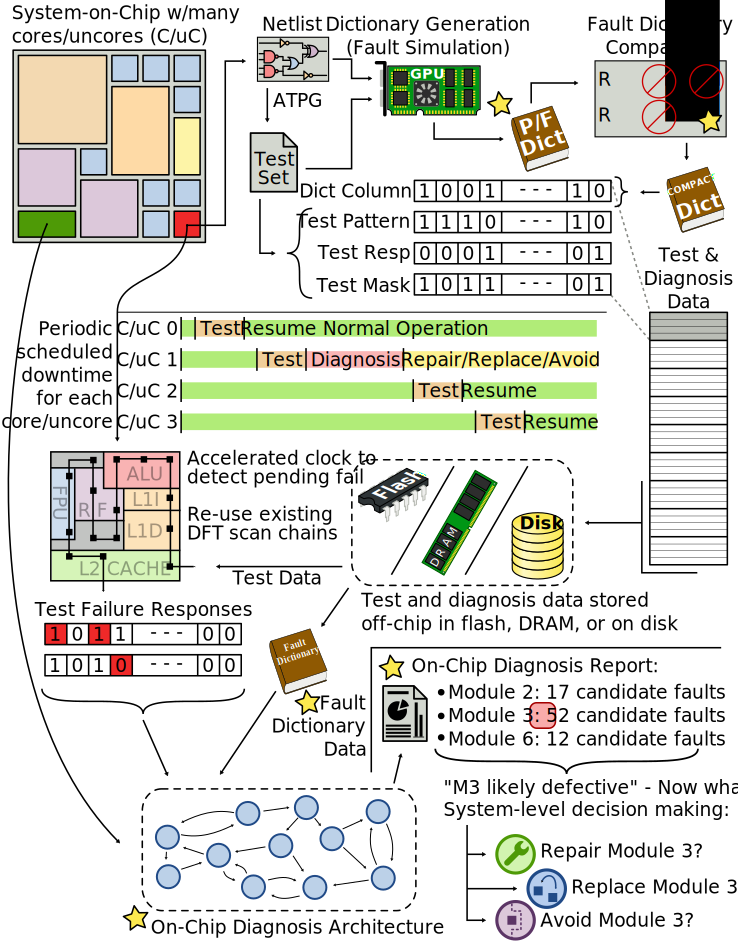
\includegraphics[width=1.0\columnwidth]{fig_intro_supergraphic}
\caption{Overall system test and diagnosis process includes several dissertation contributions (indicated by a yellow star).}
\label{fig:intro_supergraphic}
\end{figure}

Figure~\ref{fig:intro_supergraphic} shows a high-level view of these concepts.
%
While this dissertation does not accomplish everything shown (a yellow star icon indicates dissertation contributions), it is important to understand the overall process into which this dissertation fits.
%
The netlist of each System-on-Chip (SoC) core/uncore is used with Automatic Test Pattern Generation (ATPG) to generate a test set.
%
GPU-accelerated fault simulation analyzes the core/uncore netlist and test set to produce the pass/fail dictionary, further processed by dictionary compaction to produce the compacted pass/fail dictionary.
%
This pre-computed test and diagnosis data (consisting of the test pattern, test response, test mask, and fault dictionary data) is stored off-chip in flash, DRAM, or on disk.
%
The on-chip test controller~\cite{li13} schedules periodic testing downtime, for each core/uncore in the system.
%
The corresponding test data is applied to the core/uncore under test, re-using existing DFT structures such as scan chains and/or boundary scan.
%
The on-chip diagnosis architecture uses the hierarchical fault dictionary data to analyze the failing test responses to determine the set of candidate faults, grouped by repair-level module.
%
These per-module candidate fault counts are provided to the system-level for decision making, for example, to choose between repair, replacement, or avoidance of the most likely defective module(s).

\section{System Test and Diagnosis}
\label{sec:intro_system_test_and_diag}

Knowing that a system has failed (or will fail) is not sufficient to ensure robustness.
%
Beyond failure detection, there must also be a way to replace the faulty system component, repair the system, or to continue operation while avoiding the faulty circuitry.
%
One example of system repair is detailed in~\cite{li13}, where non-processor System-on-Chip (SoC) components such as cache and memory controllers (so-called \textit{uncore} components) are enhanced with self-repair capabilities.
%
The two repair techniques described in~\cite{li13} include (i) resource reallocation and sharing, where \textit{helper} components are reconfigured to share the workload of the faulty component, and (ii) sub-component logic sparing, where the design hierarchy is traversed to identify identical sub-components that could share logic spares.
%
Using both of these techniques, the authors of~\cite{li13} achieve self-repair coverage of 97.5\% with only 7.5\% area and 3\% power overhead for the OpenSPARC T2 processor design~\cite{sun11}.

Before a repair technique can be applied, however, the location of the faulty circuit must be identified.
%
Moreover, the identification process must be performed in-situ, since it is unlikely it can be accomplished off-chip without affecting system performance.
%
The process of identifying the failure location is known as \textit{diagnosis}.
%
In diagnosis, the conventional objective is to identify a fault site corresponding to the actual failure location.
%
Two categories of approaches exist for diagnosis.
%
In effect-cause diagnosis, a complete model of the design, its test-vector set, and the test response from the failing circuit are analyzed by diagnostic software to identify possible fault locations.
%
All commercial EDA vendors offer powerful software tools for diagnosing modern designs using effect-cause approaches.
%
An effect-cause approach for on-chip diagnosis is likely infeasible since the amount of memory and run-time for modern designs can be extremely large.
%
For example, merely loading the netlist image of a modern design into memory can take more than an hour.

The other approach to diagnosis is known as cause-effect, where all faults are simulated to create a cataloging or \textit{dictionary} of all possible test responses.
%
Diagnosis compares the actual circuit-failure response with all the fault-simulation responses stored in the dictionary.
%
Fault sites with a response that matches or closely matches the actual failing-circuit response are identified as likely failure locations.
%
Ideally, only one fault site is reported.

Unlike effect-cause approaches, the actual task of using a dictionary does not require a complex software analysis tool.
%
Instead, the significant task of creating the dictionary is performed only once, off-line, before the design is even fabricated, thus allowing the immense computation required to be amortized over all systems that will utilize the dictionary.
%
Performing diagnosis using a dictionary consists of lookups, which in an on-chip environment, can be efficiently accomplished by storing the dictionary in off-chip memory.

Conventional fault dictionaries are not perfect however in that they suffer from three significant drawbacks.
%
First, as mentioned, the generation time is significant.
%
This is because every fault is simulated using all test patterns (i.e., there is no fault dropping), and the complete fault response needs to be generated in the most general case.
%
Second, since the entire response for every possible fault is stored in the dictionary, its size can be huge.
%
Finally, because the dictionary size is a tremendous challenge, the fault model employed must have a limited universe (e.g., on par with the stuck-at model).
%
The consequence of using a simple fault model means however that it is much more likely that the actual circuit-failure response will differ significantly from any of the modeled fault responses stored in the dictionary.

Despite these drawbacks, dictionaries are the best choice for on-chip diagnosis since these disadvantages can be mitigated.
%
Specifically, the cost associated with dictionary generation can be amortized across the lifetimes of all the systems that will use the dictionary for on-chip diagnosis.
%
Dictionary size can be substantially reduced using conventional techniques, and by reducing the number of faults in the dictionary through a new form of collapsing that exploits the granularity of repair.
%
Additionally, advanced computational resources such as Graphics Processing Units (GPUs) can exploit the highly-parallel nature of fault simulation to drastically reduce the amount of time required for dictionary generation.
%
Finally, the failure-fault mismatch problem is handled through the use of an enhanced delay-fault model that conservatively captures the possible misbehaviors exhibited by early-life and wear-out failures without increasing the size beyond the stuck-at fault universe.

It is important to consider the differences between the goals of conventional fault diagnosis and the goals of on-chip diagnosis.
%
In conventional fault diagnosis, the focus is on process improvement or low-level design improvement via physical failure analysis (PFA) of the sites reported by diagnosis.
%
PFA requires a precise result, ideally the actual $(x, y, z)$ location of the failure.
%
The on-chip diagnosis requirements are comparatively relaxed, however, requiring localization only to the level of recovery, which is likely a much larger chip area than a single net or standard cell.
%
This relaxation of localization precision significantly reduces the size of an on-chip dictionary.


\section{On-Chip Test Framework (CASP)}
\label{sec:intro_casp}

The on-chip diagnosis work presented in this dissertation assumes the availability of a suitable on-chip test framework, specifically CASP (Concurrent Autonomous chip self-test using Stored test Patterns)~\cite{li08,li10casp,li13}.
%
This section presents an explanation of the workings of the CASP on-chip test architecture.

The overall approach employed by CASP is to periodically test core/uncore components of a SoC during runtime, without creating any user-visible system downtime.
%
The key ideas of CASP include:
\begin{itemize}
\item As opposed to random test patterns, high-quality, ATPG-generated test-vector pairs provide high fault coverage (but tests must be stored off-chip due to their size and number).
\item Small modifications to the circuit design enable the on-chip CASP controller to pause, test, and resume operation of the cores/uncores of an SoC without significantly affecting system performance.
\item Employment of a faster-than-standard clock can detect gradually-slowing defects due to aging.
\item Existing on-chip Design for Testability (DFT) structures such as scan chains, compression, etc., are utilized to perform CASP runtime test.
\item Test patterns can be updated in the field to match operational characteristics gathered over the lifetime of the system.
\end{itemize}

The core of the CASP process is the CASP controller, a finite state machine (FSM) implemented in additional hardware added to the IC design.
%
The CASP controller iterates through the following high-level steps described next and also illustrated in Figure~\ref{fig:on_chip_test_casp}.

\begin{enumerate}
\item \textbf{Scheduling} - A core/uncore is selected for the next test cycle.
%
This selection can be as simple as a round-robin approach where each core/uncore is tested in turn, or selection can be guided by usage (workload) or based on canary circuits indicating which cores/uncores are likely to need testing.
\item \textbf{Isolation} - The selected core/uncore is isolated from the rest of the system.
%
For a CPU core this typically involves stalling the execution pipeline, waiting until in-flight instructions complete, invalidating the local private cache(s), and saving critical states to shadow registers.
%
This can be significantly simplified on systems utilizing virtualization~\cite{inoue08}, where the virtual machine monitor can pause or migrate the CPU selected for testing without any hardware modifications or shadow registers.
%
For an uncore component, isolation typically involves migrating the workload of the tested uncore to a so-called ``helper'' uncore that provides some or all of the functionality of the tested uncore, enabling continued operation during test~\cite{li10}.
%
For example, since CASP does not cover memory arrays such as caches (existing resilience techniques for on-chip memories include row/column sparing, built-in self test, and error-correcting codes), when a cache controller is under test, the corresponding cache memory is still available for use.
%
A neighboring cache controller can respond to requests for data stored in the cache-under-test, provided it is made aware of the data stored there.
%
While this sharing may require additional hardware (such as enabling a cache controller to distinguish between data cached locally or in a neighboring cache), and can result in a performance degredation due to the same workloads sharing fewer active uncores, this is a better result than pausing the tasks of the uncore under test.
\item \textbf{Testing} - The high-quality test set is loaded from off-chip (flash, DRAM, or hard drive) into on-chip buffers.
%
The CASP controller sets the proper signals and states in the core/uncore under test to enable the JTAG interface that is used to load the test data into the scan chains.
%

\item \textbf{Reintegration / Recovery} - After the test phase is complete, if the core/uncore passes all tests it must be reintegrated back into the system.
%
Otherwise, apropriate recovery actions are taken for the faulty core/uncore.
%
For a non-faulty core/uncore, the isolating actions of phase two are reversed, restoring any saved state, restarting execution, and invalidating any potentially-state data from data caches.
%
For a CPU core, the execution state is restored from shadow registers, or the virtual machine OS is migrated back to the tested core (as in~\cite{inoue08}).
%
For an uncore, this may involve migrating state from the ``helper'' uncore that temporarily handled requests to the uncore under test.
\end{enumerate}

\begin{figure}[hbtp]
\centering
\includegraphics[width=\columnwidth]{on_chip_test_casp}
\caption{The CASP on-chip testing process.}
\label{fig:on_chip_test_casp}
\end{figure}

A few notes must be made as to how this architecture fits into the broader system on chip.
%
The CASP testing process (step 3 above) compares the circuit response against the expected response, for each applied test, to determine if the core/uncore is operating correctly.
%
If any failures are detected, the on-chip diagnosis process is performed using the recorded circuit responses and the diagnosis architecture presented in Chapter~\ref{chap:diag}.
%
With regard to connections between the CASP test controller and the individual cores/uncores that must be tested, there are a few details to consider.
%
First, the test controller must have access to override the control logic of each core/uncore in order to isolate it and apply the test.
%
Additionally, to perform circuit failure prediction~\cite{agarwal07}, where test pairs are applied at speeds greater than the normal system clock rate, in an effort to detect gradually-slowing gates, the test controller must have the ability to supply an accelerated clock to each testable core/uncore.
%
This is no easy feat, as significant IC routing resources are dedicated to the normal clock distribution network, and it can be a challenge to provide a secondary high-speed cross-chip clock distribution network.


\section{Transition-X (TRAX) Fault Model}
\label{sec:intro_trax}

The gate-delay fault (GDF) model~\cite{jha03} is an ideal fault model to represent the slowdown caused by early-life and wear-out failures.
%
However, the process of finding tests to detect a GDF is an optimization problem, involving searching for a sensitizable path through the gate that exhibits the minimal slack.
%
This adds undesired complexity to the already intractable test generation process.
%
The GDF model is unnecessarily more complex for an on-chip fault dictionary.
%
As an alternative, the transition fault (TF) model~\cite{jha03} is the most commonly-deployed delay fault model, widely used because it is a delay fault model with a limited fault universe.
%
While the GDF model makes no assumption about the increase in delay, the TF model assumes the delay to be larger than the slack of any sensitized path through the fault.
%
This assumption reduces complexity significantly, as any test that establishes the appropriate transition and sensitizes a path from the fault site to an output will detect a TF fault.
%
Indeed, the TF model is more tractable but is very pessimistic because it assumes that every fault will cause observable faulty behavior on all sensitized paths.%todo why is TF the most-widely deployed fault model?

There is an existing variation of the TF model, the \textit{unspecified transition fault (UTF) model}~\cite{pomeranz08}, that is a compromise between the GDF and the TF models.
%
Under the UTF model, a fault site produces an unknown value \textit{X} when activated by a transition.
%
The TRAX fault model presented here is an enhancement of the UDF model and includes fault activation due to glitches resulting from hazards, noise, etc.
%
One advantage of this fault model is that the unknown value \textit{X} captures all the possible transport-delay changes that might be exhibited by a gate affected by wear-out or early-life defects, due to the conservative propagation of the \textit{X} value.
%
Whereas the errors from a conventional transition fault could interact to increase or decrease the number of fault-effect observations (i.e., failing outputs), the \textit{X} value can only increase the number of failing outputs.
%
In other words, the set of sensitized paths with \textit{X} values will subsume the sensitized paths associated with any GDF of any delay.
%
Also, any error interaction that may occur due to the TF fault model assuming gross slowdown is also conservatively handled.

It is important to discuss further the interpretation of observed \textit{X} values at circuit outputs due to a detected TRAX fault.
%
Observed \textit{X} values from TRAX fault simulation will identify outputs that could (but not necessarily) be affected by a slowdown by a TRAX fault.
%
That is, outputs with \textit{X} values may or may not exhibit an error (depending on the level of slowdown).
%
We assume every test that detects a given TRAX fault will have at least one observed \textit{X} value, thus guaranteeing detection.
%
However, no knowledge about the timing is assumed, so it cannot be known in advance which output will have an incorrect value when a TRAX fault is detected.

%\vskip 0.2em%
\begin{figure}[hbtp]
\centering
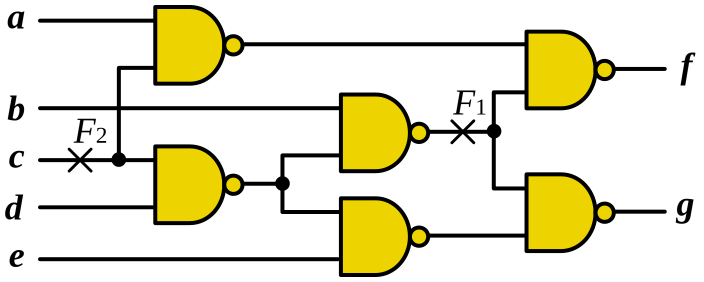
\includegraphics[width=0.7\columnwidth]{fig_c17_tf_trax}
\caption{Contrasting fault-effect propagation for the TF and TRAX models.}
\label{fig:intro_c17_tf_trax}
\end{figure}
\begin{table}[hbtp]
\renewcommand{\arraystretch}{1.2}% increase table row spacing
\centering
\begin{tabular*}{0.7\columnwidth}{@{\extracolsep{\fill}}r|r|r|c|c|c}
Fault&Fault&Two-vector test&\multicolumn{3}{c}{Output: $f g$}\\
site&type&($v_1$, $v_2$): $a b c d e$&FF&TF&TRAX\\
\hline
\multirow{2}{*}{$F_1$}&\multirow{2}{*}{STF} &$v_1: 10100$&10&10&10\\
                      &                     &$v_2: 11100$&11&10&1X\\
\hline
\multirow{2}{*}{$F_2$}&\multirow{2}{*}{STR} &$v_1: 11010$&11&11&11\\
                      &                     &$v_2: 11110$&10&11&XX\\
\end{tabular*}
\caption{Fault-free (FF) behavior of benchmark circuit c17~\cite{brglez85} (Figure~\ref{fig:intro_c17_tf_trax}) compared to TF and TRAX faults located at sites $F_1$ and $F_2$.}
\label{table:intro_tf_trax_comparison}
\end{table}
%\vskip 0.2em%

To contrast the TF and TRAX fault models, the ISCAS85 benchmark circuit c17~\cite{brglez85} is used (Figure~\ref{fig:intro_c17_tf_trax}).
%
Fault simulation is performed for TF and TRAX faults at sites $F_1$ and $F_2$, using two test-vector pairs.
%
The results of fault-effect propagation from each fault site to the circuit outputs are shown in Table~\ref{table:intro_tf_trax_comparison}.
%
The first pair of vectors activates a slow-to-fall fault at $F_1$; both the TF and TRAX produce a faulty value at output $g$.
%
In this case, both faults are detected at output $g$.
%
The second pair of vectors activates a slow-to-rise fault at $F_2$, which activates more-complex behavior and shows the difference in fault-effect propagation between TF and TRAX faults.
%
The reconvergent fanout logically masks the fault effects reaching the upper output $f$ for TF.
%
However, masking is not possible for TRAX, and both outputs take on \textit{X} values, subsuming the response of the TF.
%
The two observed \textit{X} values indicate it is possible that the actual response of a delay defect could subsume, match, or mismatch the TF response.

Since this fault model is designed to be used for diagnosis as part of a fault dictionary, attention must be paid to the computational requirements of generating such a dictionary.
%
Generating a fault dictionary using even the simplest fault model (e.g., single stuck-at) is a challenging task.
%
The task is even more daunting when using the TRAX fault model.
%
The difficulty in generating a fault dictionary is due to several factors, most notably that every fault must be simulated for all test patterns.
%
Unlike conventional fault simulation for test set evaluation, where faults are ``dropped'' after the first detection, fault dictionary generation requires full simulation results with no dropping.
%
Moreover, the complex characteristics of the TRAX fault model exacerbate the fault simulation process.
%
For example, the generalized activation conditions for the TRAX fault model involving hazards increases the complexity of fault simulation itself which means, of course, the non-dropping simulation of TRAX faults is more compute intensive.
%
As discussed later, TRAX fault simulation uses additional logic values (notably, \textit{X} and \textit{H}), which require additional memory and computation time for each gate evaluation.
%
Furthermore, the use of these additional logic values requires a complete TRAX simulation, that is, it is not possible to use the results of a simpler and faster 0/1 circuit simulator as a starting point for TRAX fault simulation.

Past efforts to accelerate fault simulation are focused around simulating in parallel and are divided into a few broad categories based on which aspect of computation is parallelized.
%
These include algorithm-parallel (\cite{agrawal87, amin97}), model-parallel (\cite{tai93, narayanan92}), and data-parallel (\cite{beece88, ozguner88, pfister82}) techniques.
%
The data-parallel techniques are further divided into fault-parallel and pattern-parallel (\cite{gulati09, parkes95, lee91}) approaches.
%
The approach presented in this work to accelerate fault simulation using GPUs uses both fault-parallel and pattern-parallel approaches for different parts of the computation.

While originally designed to speed up the highly-parallel workloads associated with 3D graphics rendering, GPUs have found new utility in the realm of high-performance parallel processing for certain types of problems, particularly for EDA-type problems~\cite{croix09}.
%
A key characteristic of the 3D graphics problem, and many other problems including fault simulation, is that very many independent calculations can be performed in parallel.
%
For example, the individual pixels of a rendered image, or the two-vector tests applied to a faulty circuit, can all be independently computed in parallel.

Although the use of GPU in EDA is relatively new, there are many publications on its use in fault simulation (\cite{gulati09, parkes95, li10, kochte10, huaweili10, gulati08, chatterjee09}).
%
All of this past work has been focused, of course, on exploiting the inherent parallelism exhibited by fault simulation.
%
What is different about the work here for dictionary construction includes the specific focus on the TRAX fault model, efficiently simulating two-vector tests, as well as various optimizations (two-input gates, a power-of-two number of logic values, etc.) targeting the specific fault simulation needs for compact dictionary generation.
%
Experiments involving various circuits, including the OpenSPARC T2 processor, demonstrate an average speed-up of nearly 8x.


\section{Hierarchical Fault Dictionary}
\label{sec:intro_dict}

In addition to the TRAX fault model, this dissertation also introduces a fault dictionary scheme optimized for performing on-chip diagnosis only to the required level of localization.
%
As previously mentioned, the only action available to an SoC at runtime is to repair, replace, or avoid a faulty module.
%
Therefore the fault dictionary needs only localize any failure(s) to the module level of the design hierarchy, hence our use of the term \textit{hierarchical fault dictionary}.

A fault dictionary for a given circuit can be conveniently viewed as a table of expected circuit responses (or some subset of the circuit response), with one row for each fault and one column for each test.
%
Each table entry is the response (or some subset) of the corresponding fault/test pair.
%
A \textit{full-response dictionary} contains the full response for each fault/test pair.
%
This dictionary can require significant storage space for modern designs.
%
As an example, the OpenSPARC T2 L2 cache write-back buffer uncore (called L2B)~\cite{sun11} contains just over 12,000 gates and uses 90 test vector pairs for test and diagnosis.
%
The full-response fault dictionary for L2B requires over 600 megabytes of storage, which is impractical for on-chip diagnosis for this relatively small circuit.
%
A variety of compaction schemes (\cite{arslan02, bernardi06, boppana94, chakravarty99, boppana96, chess99, hong07, pomeranz92}) have been developed to reduce the size of a fault dictionary, but existing schemes do not enable a sufficient level of compaction for modern designs (\cite{ryan93, boppana94}).

The TRAX hierarchical dictionary employs several techniques to reduce dictionary size.
%
First, one straightforward compaction technique is to include only faults relating to the targeted defect model (i.e., early-life and wear-out defects).
%
To this end, the TRAX fault dictionary only includes faults located at standard-cell outputs because early-life and wear-out defects affect the delay of standard cells.
%
Elimination of the remaining faults (i.e., faults located at primary inputs or fanout branches) reduces dictionary size through the elimination of dictionary rows.
%
Second, given that the system resources for on-chip test and diagnosis are necessarily limited by integrated circuit area and power budgets, it is not feasible to store the entire circuit response of every fault for every test.
%
Instead, a single bit that indicates the pass/fail outcome of a test is stored for each fault/test pair, resulting in a \textit{pass-fail dictionary}, a well-known technique for significantly reducing dictionary size at the expense of diagnostic resolution~\cite{pomeranz92}.
%
Finally, for on-chip test and diagnosis, the tested circuit (SoC core or uncore) is assumed to be partitioned into a set of modules, each of which can be independently repaired, replaced, or avoided if found to be faulty.
%
Figure~\ref{fig:intro_core_uncore_modules_faults} shows an example SoC containing three cores/uncores which themselves are composed of multiple modules, each containing TRAX faults (shown as circles within each module).
%
By recognizing that the on-chip diagnosis requirements only require fault localization to the recovery level, the diagnosis problem is significantly eased as compared to conventional approaches.

%\vskip 0.5em%
\begin{figure}[hbtp]
\centering
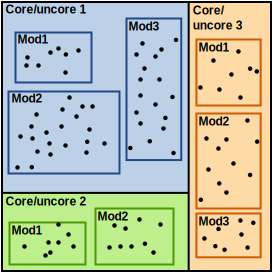
\includegraphics[width=0.4\columnwidth]{fig_core_uncore_modules_faults}
\caption{Hierarchical view of a system-on-chip (SoC) that contains multiple cores and uncores, each of which contain multiple modules.
%
Each module contains a number of faults.}
\label{fig:intro_core_uncore_modules_faults}
\end{figure}
%\vskip 0.5em%

Given this relaxation of diagnosis requirements, the concept of intra- and inter-module fault sets can lead to significant reduction in the fault count (and therefore dictionary size) necessary for accurate diagnosis.
%
For faults within the same module that are test-set equivalent (that is, those having equivalent simulation responses for all tests), all but one can be eliminated from the dictionary, as distinguishing them is unnecessary for determining a defective module.
%
Another technique to eliminate intra-module faults is called \textit{subsumption}, which is similar to the traditional concept of fault dominance, but is subtly different.
%
In brief, using the TRAX fault model and hierarchical dictionary scheme enables the elimination of any fault with a response that is subsumed by another fault in the same module.
%
A subsumed fault is no longer needed because if it fails, it would still be accurately represented in the dictionary by the subsuming fault.

%\vskip 0.5em%
\begin{table}[hbtp]
\centering
\begin{tabular*}{0.9\columnwidth}{@{\extracolsep{\fill}}cccccccl}
\toprule
Fault&Module&$T_1$&$T_2$&$T_3$&$T_4$&$T_5$&\\
\midrule
$F_1$&$M_1$&P&F&F&P&F&\\
$F_2$&$M_1$&P&F&F&P&F&Eliminated (EQU)\\
$F_3$&$M_1$&P&F&P&P&P&Eliminated (SUB)\\
$F_4$&$M_1$&F&F&P&P&F&\\
\midrule
$F_5$&$M_2$&F&F&P&P&F&\\
$F_6$&$M_2$&P&P&F&F&P&\\
\bottomrule
\end{tabular*}
\caption{TRAX fault dictionary data illustrates dictionary compaction, using equivalence and subsumption relationships to eliminate two intra-module faults.}
\label{table:intro_fault_resp}
\end{table}
%\vskip 0.2em%

Table~\ref{table:intro_fault_resp} shows an example of equivalence and subsumption fault reduction, where fault $F_2$ is eliminated via equivalence to $F_1$, and $F_3$ is eliminated because it is subsumed by both $F_1$ and $F_4$.
%
These two techniques for fault reduction are only applied to faults belonging to the same module, because repair-level diagnosis does not require distinguishing intra-module faults.
%
Applying these dictionary compaction techniques produces a \textit{collapsed pass/fail hierarchical dictionary}, which is used in the diagnosis experiments presented later.
%
For the L2B fault dictionary mentioned before, the full-response dictionary of over 600 megabytes is compacted to less than 32 kilobytes for the collapsed pass/fail dictionary, which is a reduction of over 20,000X.


\section{On-Chip Diagnosis Architecture}
\label{sec:intro_diag}

On-chip test and diagnosis using TRAX faults assume deployment of CASP (Concurrent Autonomous chip self-test using Stored Patterns)~\cite{li08}.
%
In CASP, a small amount of extra hardware is added to the chip to allow for the re-use of DFT logic for in-field test of the chip.
%
High-quality test vectors are stored in off-chip memory and are periodically loaded into the chip one vector at a time for test application and response observation.
%
The CASP process consists of four phases.
%
First, the CASP controller selects an SoC core/uncore for test.
%
Second, the selected core/uncore is taken offline and isolated from the rest of the system.
%
Third, each test is loaded from off-chip memory and applied to the isolated core/uncore, re-using existing design-for-test (DFT) scan logic.
%
Finally, once all tests are applied, the CASP controller returns the core/uncore to normal operation.
%
The recorded test responses are then provided to the on-chip diagnosis architecture for analysis and fault localization.
%
Since each core/uncore is tested and diagnosed independently, each type of core/uncore requires a separate fault dictionary, and a single dictionary is shared by each duplicated core/uncore.

The objective of on-chip diagnosis is to determine which module(s) of the core/uncore are defective, based on the observed test failures.
%
Due to the inherent nature of on-chip diagnosis, existing off-line approaches for multiple-defect diagnosis~\cite{pomeranz16,yu10,chen14} are not directly applicable.
%
Here, the previously-described TRAX hierarchical fault dictionary is used, which stores a single bit for each fault-test pair, indicating if the corresponding fault is detected by the corresponding test.
%
The TRAX dictionary is used in conjunction with the pass/fail test response to produce a list of potentially responsible ``candidate'' faults.
%
Specifically, starting with a list of all TRAX faults within the tested core/uncore dictionary, each failing test response is used one at a time to eliminate any faults that are not detectable by that failing test.
%
This is an instance of Tester-Fail/Simulation-Pass (TFSP) and triggers the elimination of the corresponding fault.
%
After all test responses are processed, what remains is a list of candidate TRAX faults compatible with the observed behavior.

Each fault in the list of candidate TRAX faults belongs to a specific hierarchal module of the core/uncore.
%
The candidate fault list is analyzed to count the number of candidate faults belonging to each module, resulting in a per-module candidate fault count.
%
These fault counts are used to determine which module or modules are likely defective.

A scalable on-chip diagnosis architecture is developed to use the hierarchical dictionary to localize failures only to the required level.
%
Diagnosis hardware scaled to the size of one of the largest analyzed circuits, NCU from the OpenSPARC T2 design, requires between 22,000 - 26,000 clock cycles (depending on the desired scaling) for performing diagnosis.
%
Hardware requirements range between 38,000 - 245,000 additional gates, corresponding to between 0.0077\% - 0.0491\% estimated area overhead.

\section{Multiple Defect Diagnosis}
\label{sec:intro_multi}

The TRAX fault model is designed to capture the arbitrary slowdown exhibited by a single early-life or wear-out failure.
%
Due to the very nature of the targeted failures, it is likely however that more than one failure will be present.
%
Given the conservative propagation properties of the unknown value \textit{X}, the use of the TRAX-based hierarchical dictionary can remain effective even in the presence of multiple faults.
%
This is particularly the case in the context of the targeted failure modes (early-life and wear-out failures) and the relaxed diagnostic requirements (fault localization only to the recovery level).

In Chapter~\ref{chap:multi}, an empirical analysis is performed to determine the effectiveness of the TRAX-based hierarchical fault dictionary for on-chip diagnosis, when faced with multiple runtime failures.

\section{Benchmark and Test Circuits}
\label{sec:intro_benchmark_and_test_circuits}

Measuring dictionary size reduction due to fault elimination requires access to designs that exhibit module-level hierarchy.
%
The hierarchical versions of the ISCAS85 benchmark circuits~\cite{brglez85} produced by the University of Michigan~\cite{hansen99} serve this purpose well since many of the benchmarks have been reverse engineered to at least two levels of hierarchy.
%
Additionally, three other circuit sources are utilized.
%
First, several circuits are taken from the ITC99 benchmark set~\cite{corno99}.
%
Second, two sub-circuits are taken from the freely-available OpenSPARC T2 processor design~\cite{sun11}, the previously-mentioned L2 cache write-back buffer uncore (L2B), and the Non-Cachable Unit (NCU) that decodes and directs I/O addresses.
%
Third, five circuits are taken from the EPFL combinational benchmarks suite~\cite{epfl}.
%
The non-ISCAS circuits are not pre-partitioned into a module-level hierarchy and are instead partitioned into ten modules using graph clustering and partitioning software~\cite{dhillon07}.
%
In our experiments, we equate the second-level modules of the circuits to the level of repair.
%
In other words, diagnostic precision has to be only achieved at the second level of the hierarchy within these circuits.
%
Details of the test patterns generated using a commercial ATPG tool are shown in Table~\ref{table:intro_circuit_details}.
%
As it does not support the TRAX fault model, the commercial ATPG tool is configured to generate test vector pairs targeting the transition fault (TF) model.
%
As will be explained in Chapter~\ref{chap:trax}, the activation conditions of a TRAX fault are a superset of the activation conditions of a transition fault, meaning that ATPG targeting transition faults produces a test set also effective at detecting TRAX faults.

%\vskip 0.5em%
\begin{table}[hbtp]
\center
\begin{tabular*}{0.8\columnwidth}{@{\extracolsep{\fill}}rrrr}
\toprule
Benchmark   &Transition faults     &Test pairs &Fault coverage\\
\midrule
c432        &316        &37         &99.05\%\\
c499        &456        &71         &100.00\%\\
c1355       &1,028      &106        &99.51\%\\
c1908       &578        &64         &99.65\%\\
c2670       &1,996      &67         &96.69\%\\
c3540       &2,674      &128        &99.25\%\\
c5315       &4,308      &85         &100.00\%\\
c7552       &5,530      &84         &98.63\%\\
\midrule
b12         &1,880      &80         &100.00\%\\
b14\_opt    &10,694     &345        &99.97\%\\
b14         &19,534     &657        &99.67\%\\
b15         &16,734     &407        &97.39\%\\
b17\_opt    &45,514     &600        &98.38\%\\
b18\_opt    &139,826    &704        &99.71\%\\
b22         &59,568     &554        &99.69\%\\
\midrule
L2B         &24,444     &90         &99.99\%\\
NCU         &67,124     &211        &99.95\%\\
\midrule
epflDiv     &203,206    &612        &99.25\%\\
epflMult    &101,008    &77         &99.96\%\\
epflSqrt    &82.084     &161        &91.91\%\\
epflSquare  &70,984     &79         &100.00\%\\
epflMemCtrl &165,076    &1,276      &99.84\%\\
\bottomrule
\end{tabular*}
\caption{ATPG details for benchmark circuits, including the number of transition faults, number of test pairs, and fault coverage.}
\label{table:intro_circuit_details}
\end{table}
%\vskip 0.5em%


\section{Dissertation Organization}
\label{sec:intro_dissertation_organization}


The rest of this dissertation is organized as follows: Chapter~\ref{chap:trax} details the TRAX fault model, including comparisons with existing fault models.
%
Chapter~\ref{chap:trax} also describes the GPU-accelerated fault simulator developed for specifically simulating TRAX faults in an efficient manner.
%
Chapter~\ref{chap:dict} describes the hierarchical dictionary and investigates its performance for a variety of benchmark circuits.
%
The on-chip fault diagnosis architecture is detailed in Chapter~\ref{chap:diag}.
%
The combination of the TRAX fault model, hierarchical dictionary, and on-chip diagnosis architecture is also evaluated in Chapter~\ref{chap:diag} using defect injection and diagnosis experiments.
%
Chapter~\ref{chap:multi} evaluates the efficacy of on-chip diagnosis for multiple injected defects.
%
Finally, Chapter~\ref{chap:conclusions} concludes the dissertation and includes direction for future work.
